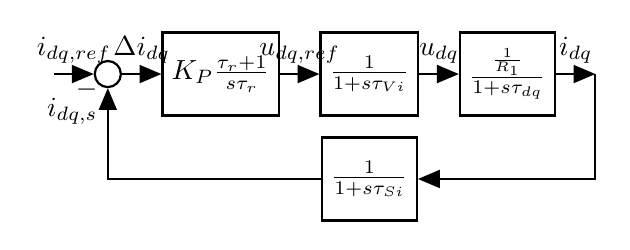
\begin{tikzpicture}[auto, thick, node distance=0.5cm, >=triangle 45]
% Definition of blocks:
\usetikzlibrary{positioning,arrows,calc}
\tikzset{%
  block/.style    = {draw, thick, rectangle, minimum height = 3em, minimum width = 2em, node distance = 0.5cm},
  sum/.style      = {draw, circle, node distance = 0.5cm}, % Adder
  input/.style    = {coordinate}, % Input
  output/.style   = {coordinate} % Output
}
\draw
	node [input, name=i_ref] {}
	node [sum, right= of i_ref] (sum1) {}
	node [block, right=of sum1] (regler) {$K_\mat{P}\frac{\tau_\mat{r}+1}{s\tau_\mat{r}}$}
	node [block, right=of regler] (umrichter) {$\frac{1}{1+s\tau_\mat{Vi}}$}
	node [block, right=of umrichter] (pmsm) {$\frac{\frac{1}{R_\mat{1}}}{1+s\tau_\mat{dq}}$}
	node [block, below=0.25cm of umrichter] (sensor) {$\frac{1}{1+s\tau_\mat{Si}}$}
	node [output, right=0.5cm of pmsm  ](i_dq){}
;
	\draw[->](i_ref) -- node {$i_\mat{dq,ref}$}(sum1);	
	\draw[->](sum1) -- node {$\Delta i_\mat{dq}$}(regler);
	\draw[->](regler) -- node {$u_{dq,ref}$}(umrichter);
	\draw[->](umrichter) -- node {$u_\mat{dq}$}(pmsm);
	\draw[->](pmsm) -- node {$i_\mat{dq}$}(i_dq);
	\draw[->]($(pmsm.east) + (0.5,0) $) |- node[very near end] {} (sensor);
	\draw[->](sensor) -| node[pos=0.99] {$-$} node[very near end] {$i_\mat{dq,s}$} (sum1);
	
	
\end{tikzpicture}